%% Charlie Redmon
%% 20170913
%% SEM path diagram: exploratory factor analysis model

% standalone class for individual image to be included in a document
% border=15pt controls the whitespace padding around the diagram
\documentclass[border=15pt]{standalone}

% load custom style configurations from separate file
%% ------------------------------------------------------------
%% Charlie Redmon
%% 20170923
%% semTikzStyle.tex: style configurations for SEM path diagrams
%% ------------------------------------------------------------

\usepackage{tikz}

% observed variable
\tikzstyle{ov}=[shape=rectangle,
                draw=black!80,
                minimum height=0.6cm,
                minimum width=0.6cm,
                thick]

% response variable
\tikzstyle{av}=[shape=rectangle,
                draw=black!80,
                fill=black!10,
                minimum height=0.6cm,
                minimum width=0.6cm,
                thick]

% latent variable
\tikzstyle{lv}=[shape=circle,
                draw=black!80,
                thick,
                minimum width=1cm]

% correlations
\tikzstyle{lcor}=[bend left=30, dashed]
\tikzstyle{rcor}=[bend right=30, dashed]

% self-loops (for variance)
\tikzstyle{lloop}=[loop left, 
                   out=210, 
                   in=150, 
                   distance=0.3cm,
                   densely dotted]

\tikzstyle{rloop}=[loop right, 
                   out=30, 
                   in=-30, 
                   distance=0.3cm,
                   densely dotted]

\tikzstyle{aloop}=[loop above, 
                   out=60, 
                   in=120, 
                   distance=0.3cm,
                   densely dotted]

\tikzstyle{bloop}=[loop below, 
                   out=-60, 
                   in=-120, 
                   distance=0.3cm,
                   densely dotted]




\begin{document}

%% ">=stealth" sets the arrow head style
%% "semithick" sets the line width (0.6 pt)
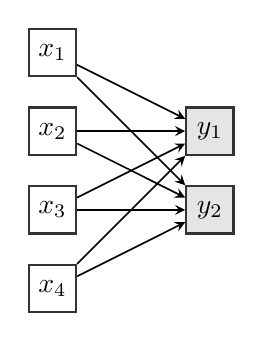
\begin{tikzpicture}[>=stealth,semithick]

% predictor nodes (x)
\node[ov] (x1) {$x_{1}$};
\node[ov] (x2) [below of=x1]  {$x_{2}$};
\node[ov] (x3) [below of=x2]  {$x_{3}$};
\node[ov] (x4) [below of=x3]  {$x_{4}$};

% response node (y)
\begin{scope}[xshift=2cm]
\node[av] (y1) at (0,-1)      {$y_1$};
\node[av] (y2) [below of=y1]  {$y_2$};
\end{scope}

% paths (arrows) between x's and y1
\path[->] (x1) edge node[above,scale=0.6] {} (y1)
          (x2) edge node[above,scale=0.6] {} (y1)
          (x3) edge node[above,scale=0.6] {} (y1)
          (x4) edge node[above,scale=0.6] {} (y1);
% paths (arrows) between x's and y2
\path[->] (x1) edge node[above,scale=0.6] {} (y2)
          (x2) edge node[above,scale=0.6] {} (y2)
          (x3) edge node[above,scale=0.6] {} (y2)
          (x4) edge node[above,scale=0.6] {} (y2);
\end{tikzpicture}


\end{document}